\documentclass[12pt]{article}

\usepackage{graphicx} 
\usepackage{fullpage}
\usepackage{amsfonts,amssymb,amsmath}
\usepackage{float}
\usepackage[most]{tcolorbox}
\usepackage[dvipsnames]{xcolor}
\numberwithin{equation}{section}
\usepackage[italian]{babel}
\usepackage{hyperref}
\usepackage{mdframed}
\usepackage{siunitx}
\usepackage{enumerate}
\usepackage{enumitem}
\usepackage{cancel}
\usepackage{accents}
\usepackage{svg}
\usepackage{mathtools}
\usepackage[a4paper,margin=2cm]{geometry}
\DeclarePairedDelimiter\angular{\langle}{\rangle}
\DeclarePairedDelimiter\bigangular{\bigg\langle}{\bigg\rangle}
\usepackage[thinc]{esdiff}
\usepackage{caption}
\usepackage{csquotes}
\usepackage[backend=biber,style=numeric, sorting=none]{biblatex}
\setlength{\parindent}{15pt}
\newcommand{\dd}{\mathrm{d}}
\setlength{\parskip}{0pt}
\usepackage{fontspec}

\setmainfont{Calibri}[
    Path = ./Fonts/,
    Extension = .ttf,
    UprightFont = calibri,
    BoldFont = calibri_bold,
    ItalicFont = calibri_italic,]

\title{Relazione Laboratorio di Circuiti}
\author{Serena Miari, Davide Rizzi}
\date{15/05/2026}

\begin{document}

\maketitle

\maketitle

\section{Abstract}

\section{Introduzione}

Nell'esperienza di laboratorio è stato progettato un circuito notch (filtro elimina banda)  RLC serie e ne è stato verificato il comportamento atteso.

Un circuito notch è un circuito elettronico che lascia passare tutte le frequenze, bloccandone o attenuandone solo una specifica [frase copiata da AI overview da modificare]. Nel circuito realizzato, la frequenza filtrata teorica era XXX.

\section{Apparato sperimentale e svolgimento}

L'apparato sperimentale utilizzato si compone di una scheda Elvis II, un multimetro digitale, un oscilloscopio, tre resistenze, un condensatore, un induttore, e un microfono.
In particolare, si è fatto uso degli strumenti soft front panel della scheda Elvis II: NI Elvis II Digital Multimeter e NI Elvis II Function Generator. Il primo è stato usato per misurare valori di induttanza, capacità e resistenza, il secondo per generare onde sinusoidali. 
I valori di capacità e induttanza sono stati scelti in modo che il grafico della frequenza fosse il più simmetrico possibile rispetto al notch.

\begin{figure}[H]
    \centering
    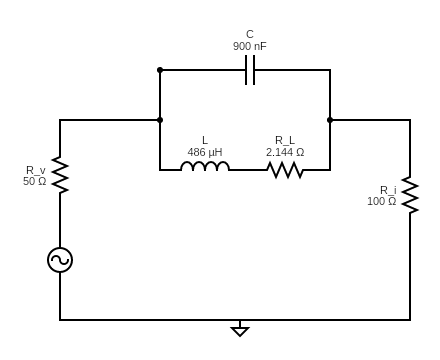
\includegraphics[width=0.5\linewidth]{Images/circuit(2).png}
    \caption{\textit{Schema del circuito notch. Sono riportati i valori di: resistenza interna del generatore ($R_v$), condensatore (C), induttore (L), resistenza interna dell'induttore ($R_L$), e di una delle resistenze utilizzate ($R_i$).}}
    \label{fig:placeholder}
\end{figure}


Inizialmente, è stato realizzato sulla breadboard Elvis II il circuito notch in figura 1. Come si può osservare, FGen è collegato al condensatore e all'induttore in parallelo. Questi sono collegati in serie con la resistenza, a sua volta collegata al ground. Sono stati utilizzati due canali di acquisizione, i cui canali negativi sono stati entrambi collegati al ground; uno dei canali positivi è stato collegato prima della resistenza e uno dopo il generatore. 

E' stato osservato il comportamento del circuito con oscilloscopio da banco, usando function generator tramite sweep in frequenza, ed è stato verificato che vi fosse abbattimento dell'ampiezza del voltaggio intorno alla frequenza di notch.
Per effettuare una successiva analisi, sono stati acquisiti tre set di dati durante sweep in frequenza: 1) l'ampiezza di voltaggio in funzione del tempo, 2) l'ampiezza di voltaggio in funzione della frequenza, e 3) la fase del voltaggio in funzione della frequenza.

Infine, è stato sostituito il generatore di tensione sinusoidale con un microfono e sono stati acquisiti ulteriori dati per osservare l'abbattimento in corrispondenza della frequenza di notch. 
L'input e il ground del microfono sono stati collegati rispettivamente ai 5 Volt e al ground della scheda Elvis, mentre l'output è stato collegato al resto del circuito in maniera analoga ad FGen.

\section{Risultati e discussione}

Nella tabella 1 sono riportati i valori nominali e misurati dal multimetro digitale della scheda Elvis del condensatore, dell'induttore, della resistenza interna dell'induttore, e di tre resistenze distinte \footnote{Per il calcolo delle incertezze associate alla misura delle resistenze mediante multimetro, si veda l'Appendice~\ref{app:Incertezze}.}.


Il valore della frequenza filtrata teorica, dipendente dall'induttore e dal condensatore, era 7292.29 Hz, mentre il valore atteso calcolato a partire dai valori reali, e dipendente in aggiunta dalla resistenza interna dell'induttore, 7575.92 Hz.

\begin{table}[H]
\centering
\begin{tabular}{||c | c | c ||} 
 \hline
 & Valore nominale & Valore misurato da multimetro \\ [0.5ex] 
 \hline\hline
 Condensatore & 1 $ \mu F$ & (0.902 $\pm$ 0.009) $ \mu F$ \\
 \hline
 Induttore & 470 $ \mu H$ & (486 $\pm$ 5) $ \mu H$ \\ 
 \hline
 $R_{L}$ & 2.5 $ \Omega $ & (2.14 $\pm$ 0.03) $ \Omega $ \\
 \hline
 $R_{1}$ & 100 $ \Omega $ & (100.31 $\pm$ 0.05) $\Omega$ \\
 \hline
 $R_{2}$ & 330 $\Omega$& (329.02 $\pm$ 0.08) $\Omega$ \\ 
 \hline
 $R_{3}$ & 560 $\Omega$ & (558.06 $\pm$ 0.06) $\Omega$ \\
 \hline
\end{tabular}
\caption{\textit{Valori nominali e misurati dal multimetro della scheda Elvis del condensatore, dell'induttore, della resistenza interna dell'induttore, e di tre resistenze distinte.}}
\end{table}


\begin{equation}
    Q = \frac{1}{R} \sqrt{\frac{L}{C}}=\frac{1}{RC \omega_0}
\end{equation}


\subsection{Fit}

A partire dai set di dati ricavati, abbiamo potuto effettuare una serie di analisi al fine di  caratterizzare il comportamento del nostro circuito. 

\begin{figure}[H]
    \centering
    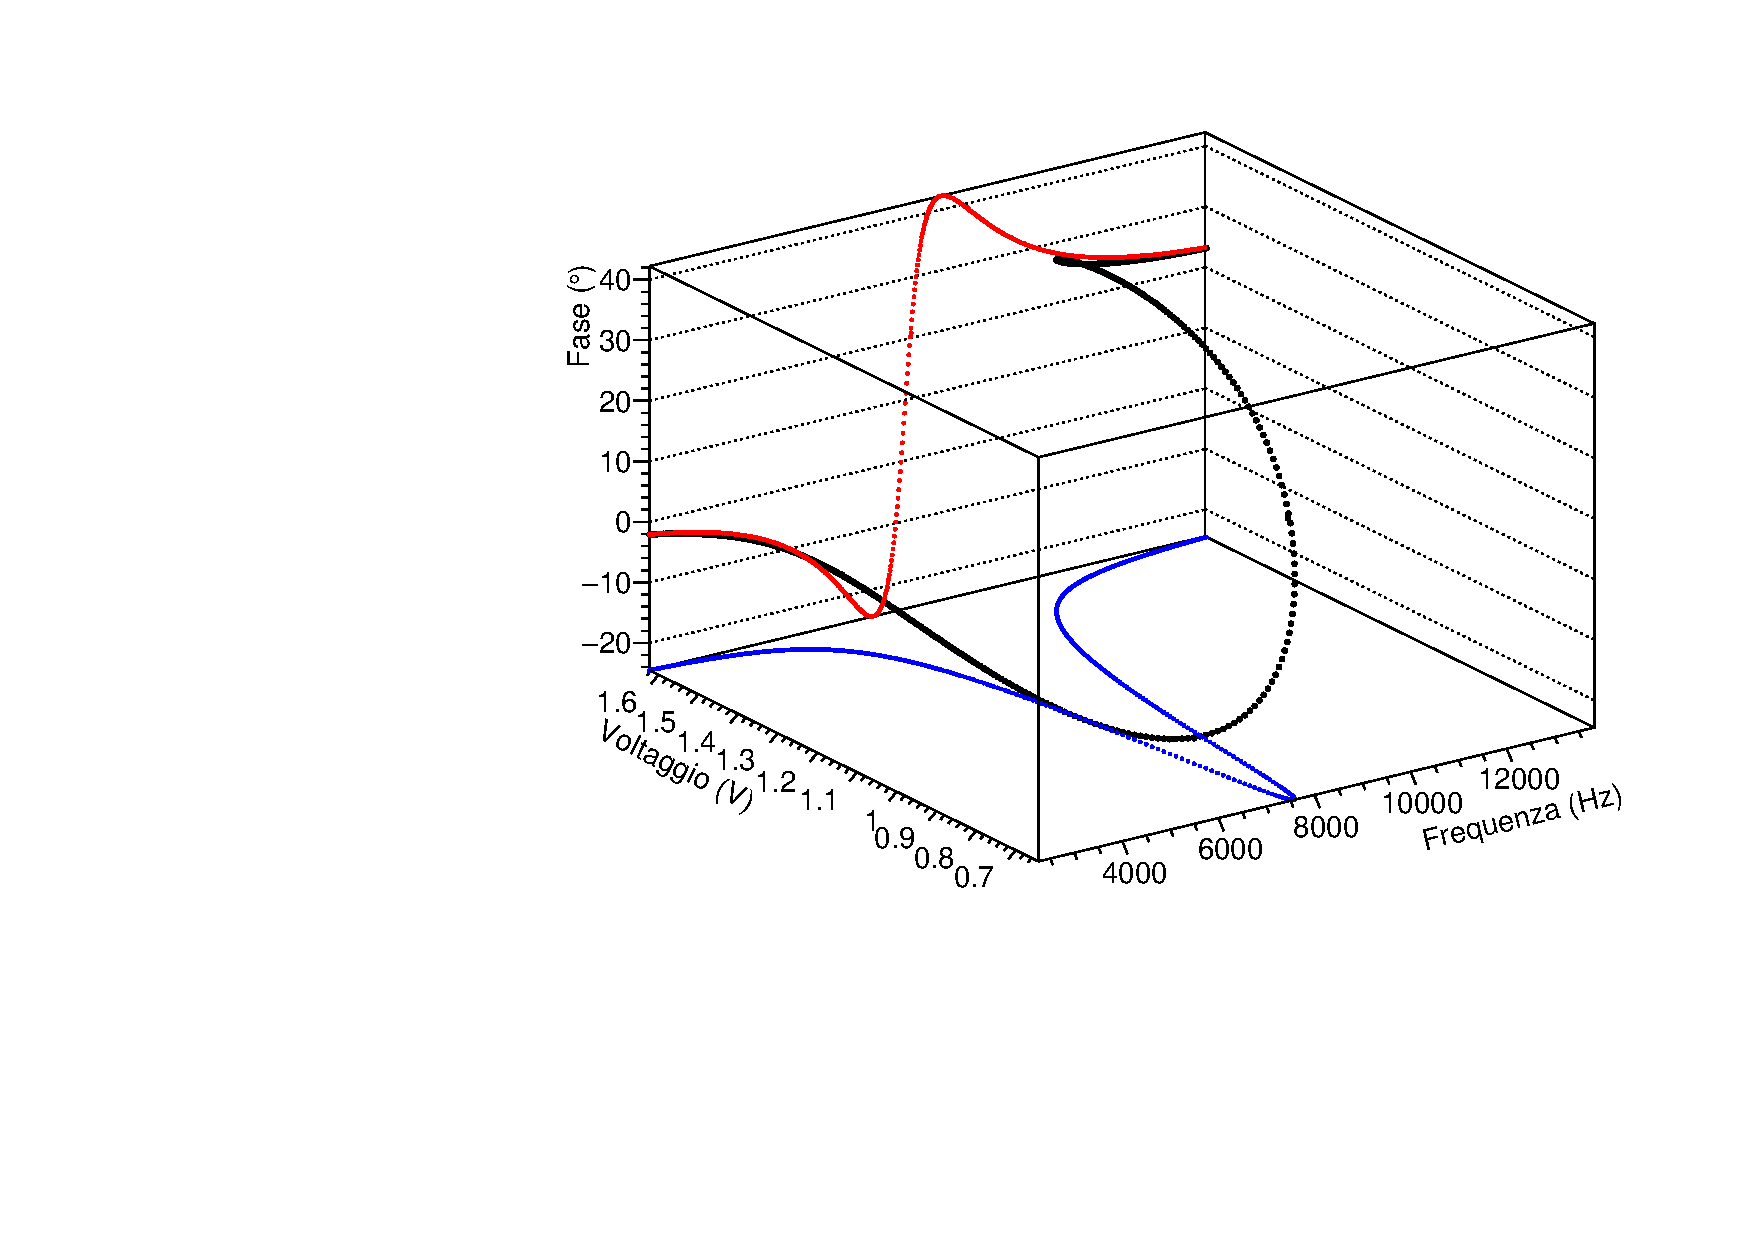
\includegraphics[width=0.5\linewidth]{Images/3D_graph.pdf}
    \caption{\textit{Grafico di dispersione del valore dell'ampiezza di voltaggio (V) e della differenza di fase ( $^{\circ}$) tra generatore e capi della resistenza in funzione della frequenza. Sul piano Hz-V, la linea blu indica l'andamento dell'ampiezza del voltaggio ai capi della resistenza in funzione della frequenza; sul piano Hz-$^{\circ}$ , è graficato in rosso l'andamento della differenza di fase tra il generatore e i capi della resistenza.}}
    \label{fig:placeholder}
\end{figure}

Come si nota dal grafico (LABEL FIGURA), il valore dell'ampiezza del voltaggio subisce uno smorzamento attorno alla frequenza di notch per poi assestarsi a un valore di regime nelle code. Questo indica che il filtro è effettivamente selettivo attorno a una specifica frequenza. Come ci si aspetta, la fase subisce una rapida inversione in corrispondenza della frequenza di notch, per poi assestarsi a un valore in modulo uguale, ma con segno opposto a quello iniziale. Il grafico della differenza di fase, rispetto ad un modello ideale, risulta traslato verticalmente a causa di un offset dovuto alla non idealità del circuito.

In un'ulteriore analisi dei dati abbiamo verificato la coerenza dei dati sperimentali raccolti, con il modello teorico atteso.

\begin{figure}[H]
    \centering
    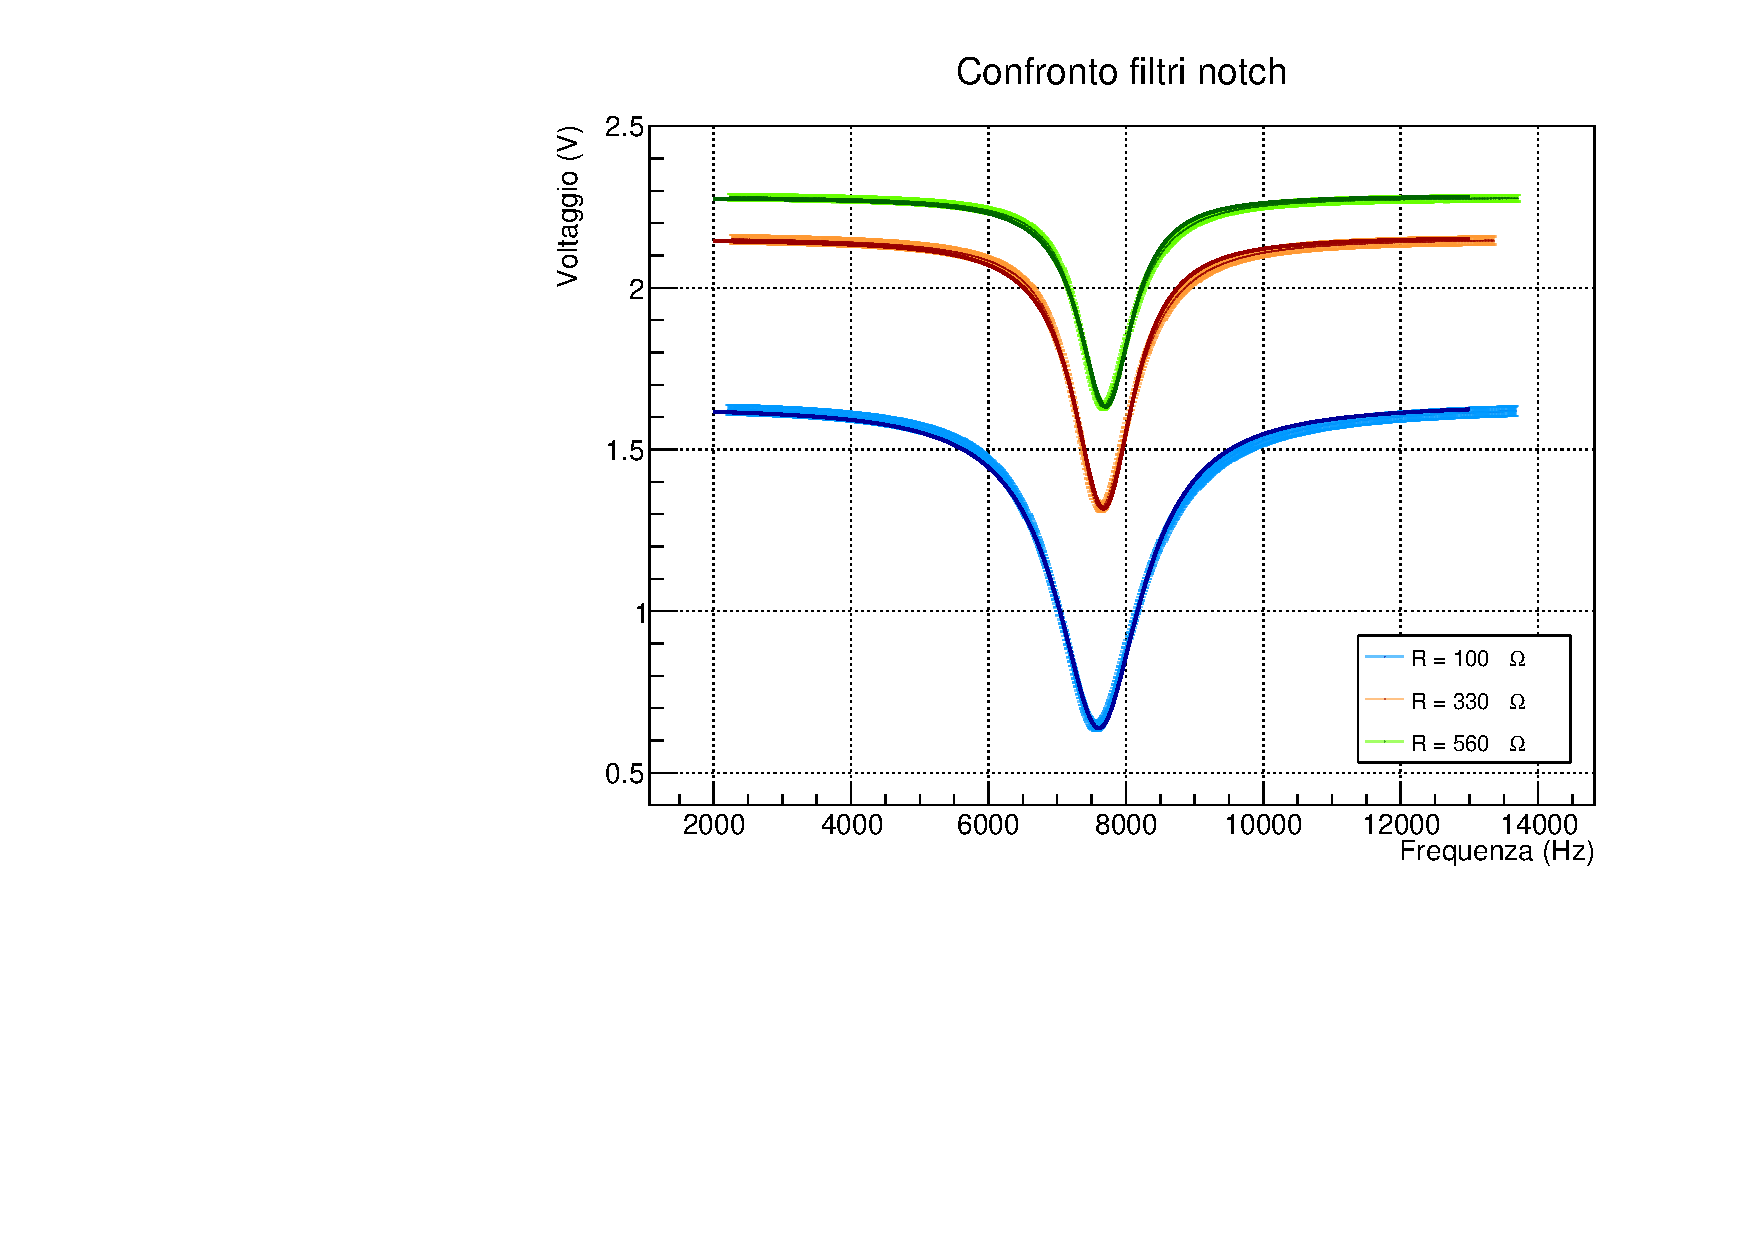
\includegraphics[width=0.8\linewidth]{Images/multi_fit.pdf}
    \caption{Enter Caption}
    \label{fig:placeholder}
\end{figure}
I dati raccolti sono stati fittati rispetto alla funzione dell'ampiezza del voltaggio ai capi della resistenza nel caso non ideale, quindi tenendo conto delle resistenze interne di generatore e induttore. La funzione di fit è la seguente:

\begin{equation}
    |V(R)| =  |V_{0}| \frac{R \sqrt{(1-w^2LC)^2+(wCR_{L})^2}}{\sqrt{[(R_{V}+R)(1-w^2LC)+R_{L}]^2+\{w[L+CR_{L}(R_{V}+R)]\}^2}} \footnote{Per il calcolo completo, si veda l'Appendice~\ref{app:Dimostrazione}.}
\end{equation}

La funzione presenta 6 parametri: resistenza del circuito ($R$), resistenza del generatore ($R_V$), induttanza ($L$), resistenza dell'induttanza ($R_L$), capacità ($C$) e ampiezza del voltaggio del generatore $|V_0|$. 

\begin{table}[H]
\centering
\begin{tabular}{||c | c | c | c | c | c ||} 
 \hline
  & Valore Nominale ($\Omega$) & Valore da Fit ($\Omega$)& Freq. Teorica (Hz) & Freq. Reale (Hz) & $\widetilde{\chi}^2$ \\ [0.5ex] 
 \hline\hline
 $R_{1}$ & 100 &  99.9 $\pm$ 0.6 & 7575.92 $\pm$ err. & 7565.08 & 1.0304\\
 \hline
 $R_{2}$ & 330 &  330.6 $\pm$ 1.8 & 7575.92 & 7640.15 & 0.9936\\ 
 \hline
 $R_{3}$ & 560 & 560 $\pm$ 3 & 7575.92 & 7670.14 & 0.9591\\
 \hline
\end{tabular}
\caption{\textit{Valori del Chi2 ridotto nelle diverse configurazioni di resistenza del filtro. La frequenza teorica è calcolata mediante formula (nel caso reale) sulla base dei valori reali delle componenti del circuito e l'incertezza associata è massima. La frequenza reale è ricavata dai dati sperimetali come il valore di frequenza del punto con ampiezza di voltaggio minore.}}
\label{tab:risultati_notch}
\end{table}


\subsection{Microfono}

\begin{figure}[H]
    \makebox[\textwidth][c]{
        \begin{minipage}{0.38\textwidth}
            \centering
            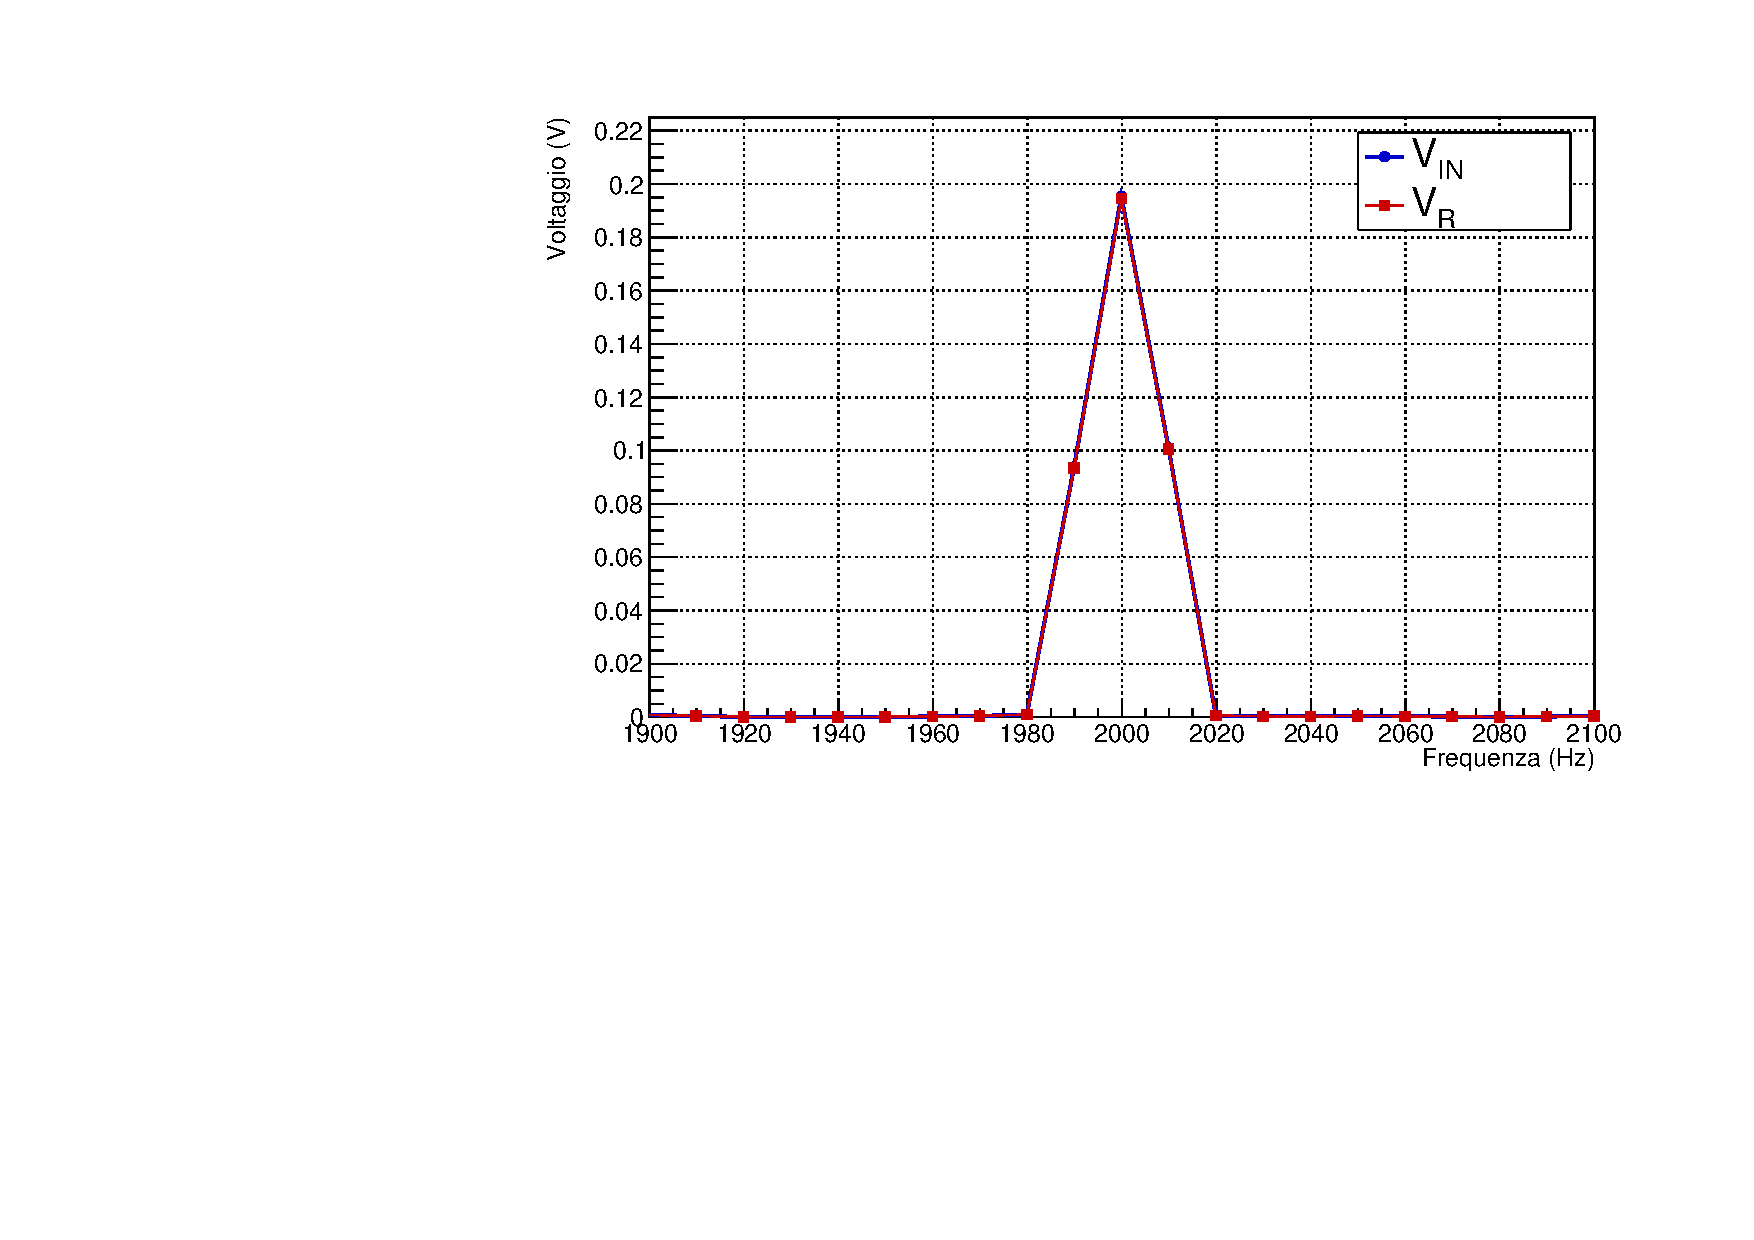
\includegraphics[width=\linewidth]{Images/Mic(2).pdf}
            \label{fig:1}
        \end{minipage}\hfill
        \begin{minipage}{0.38\textwidth}
            \centering
            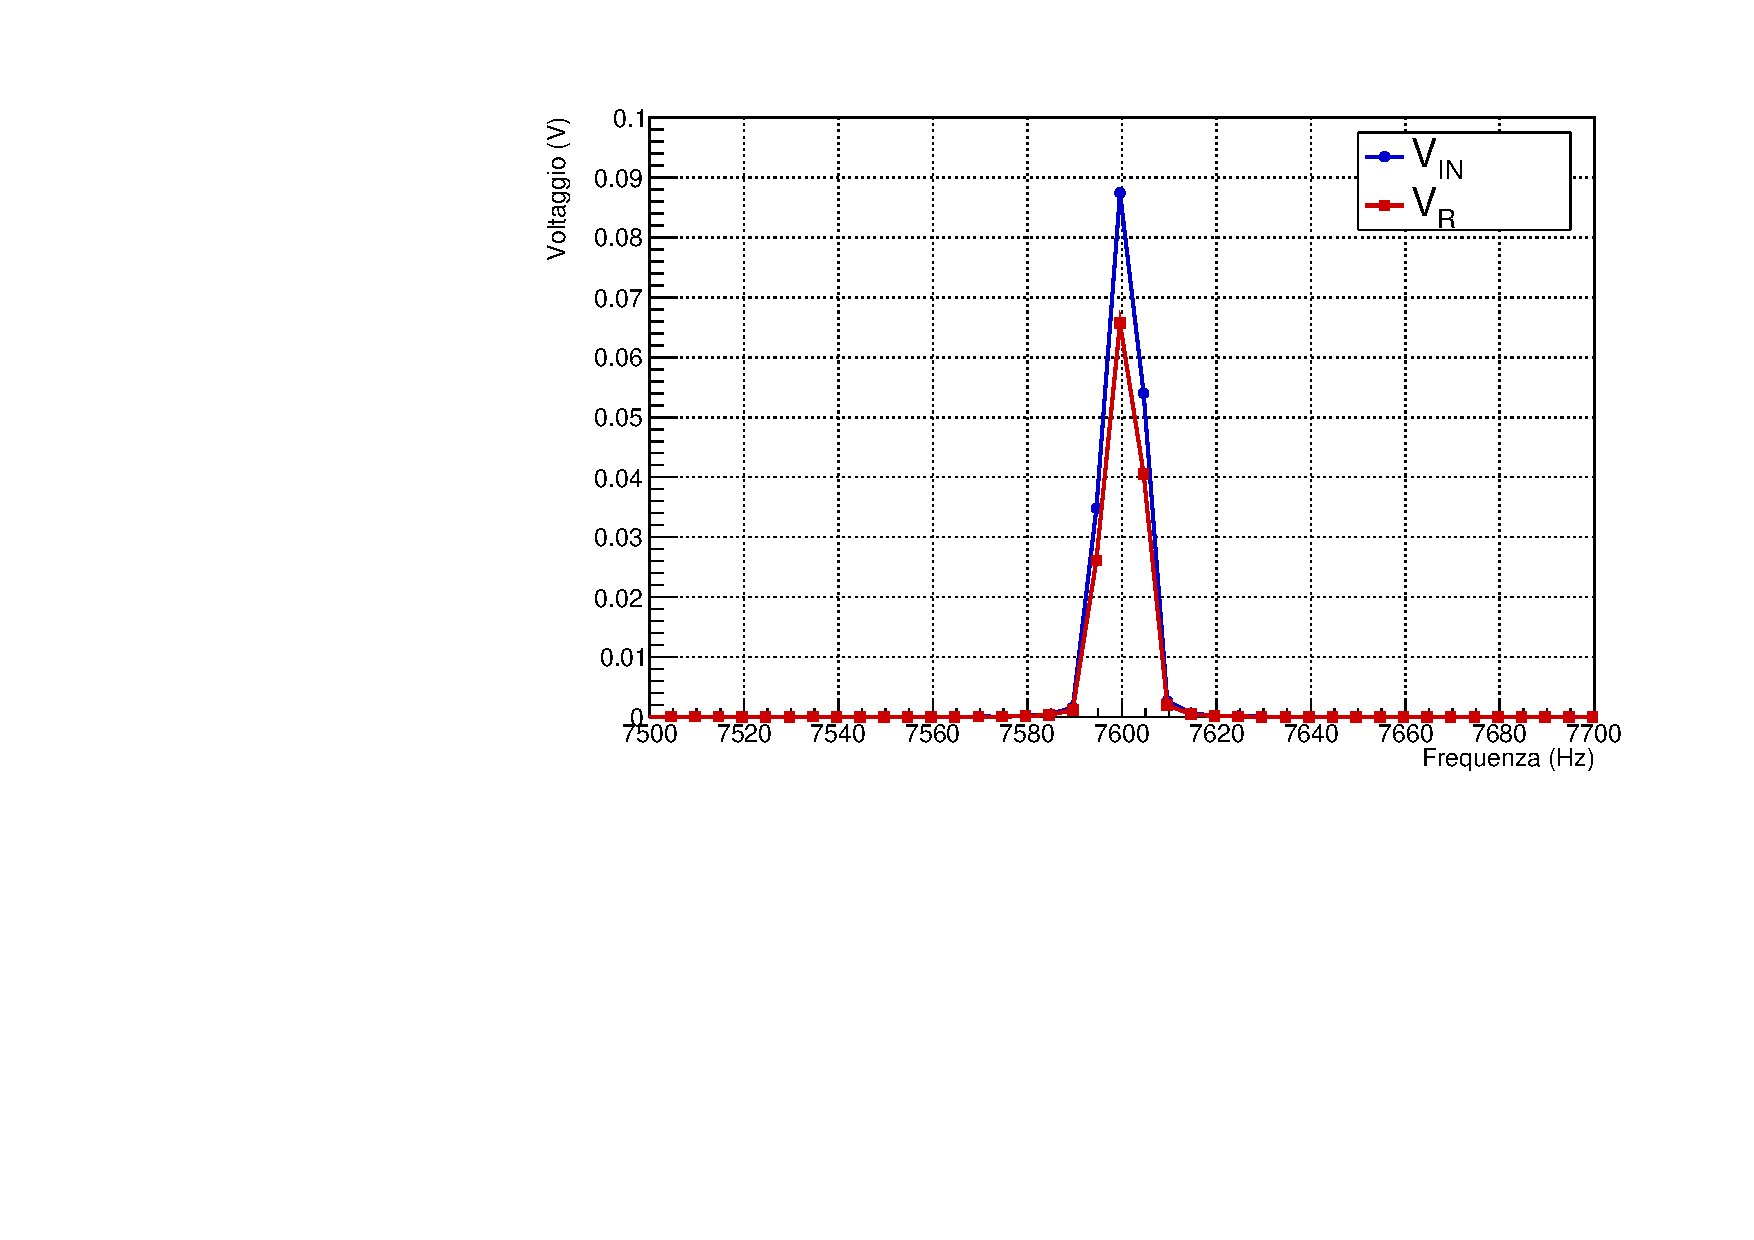
\includegraphics[width=\linewidth]{Images/Mic(7.6).pdf}
            \label{fig:2}
        \end{minipage}\hfill
        \begin{minipage}{0.38\textwidth}
            \centering
            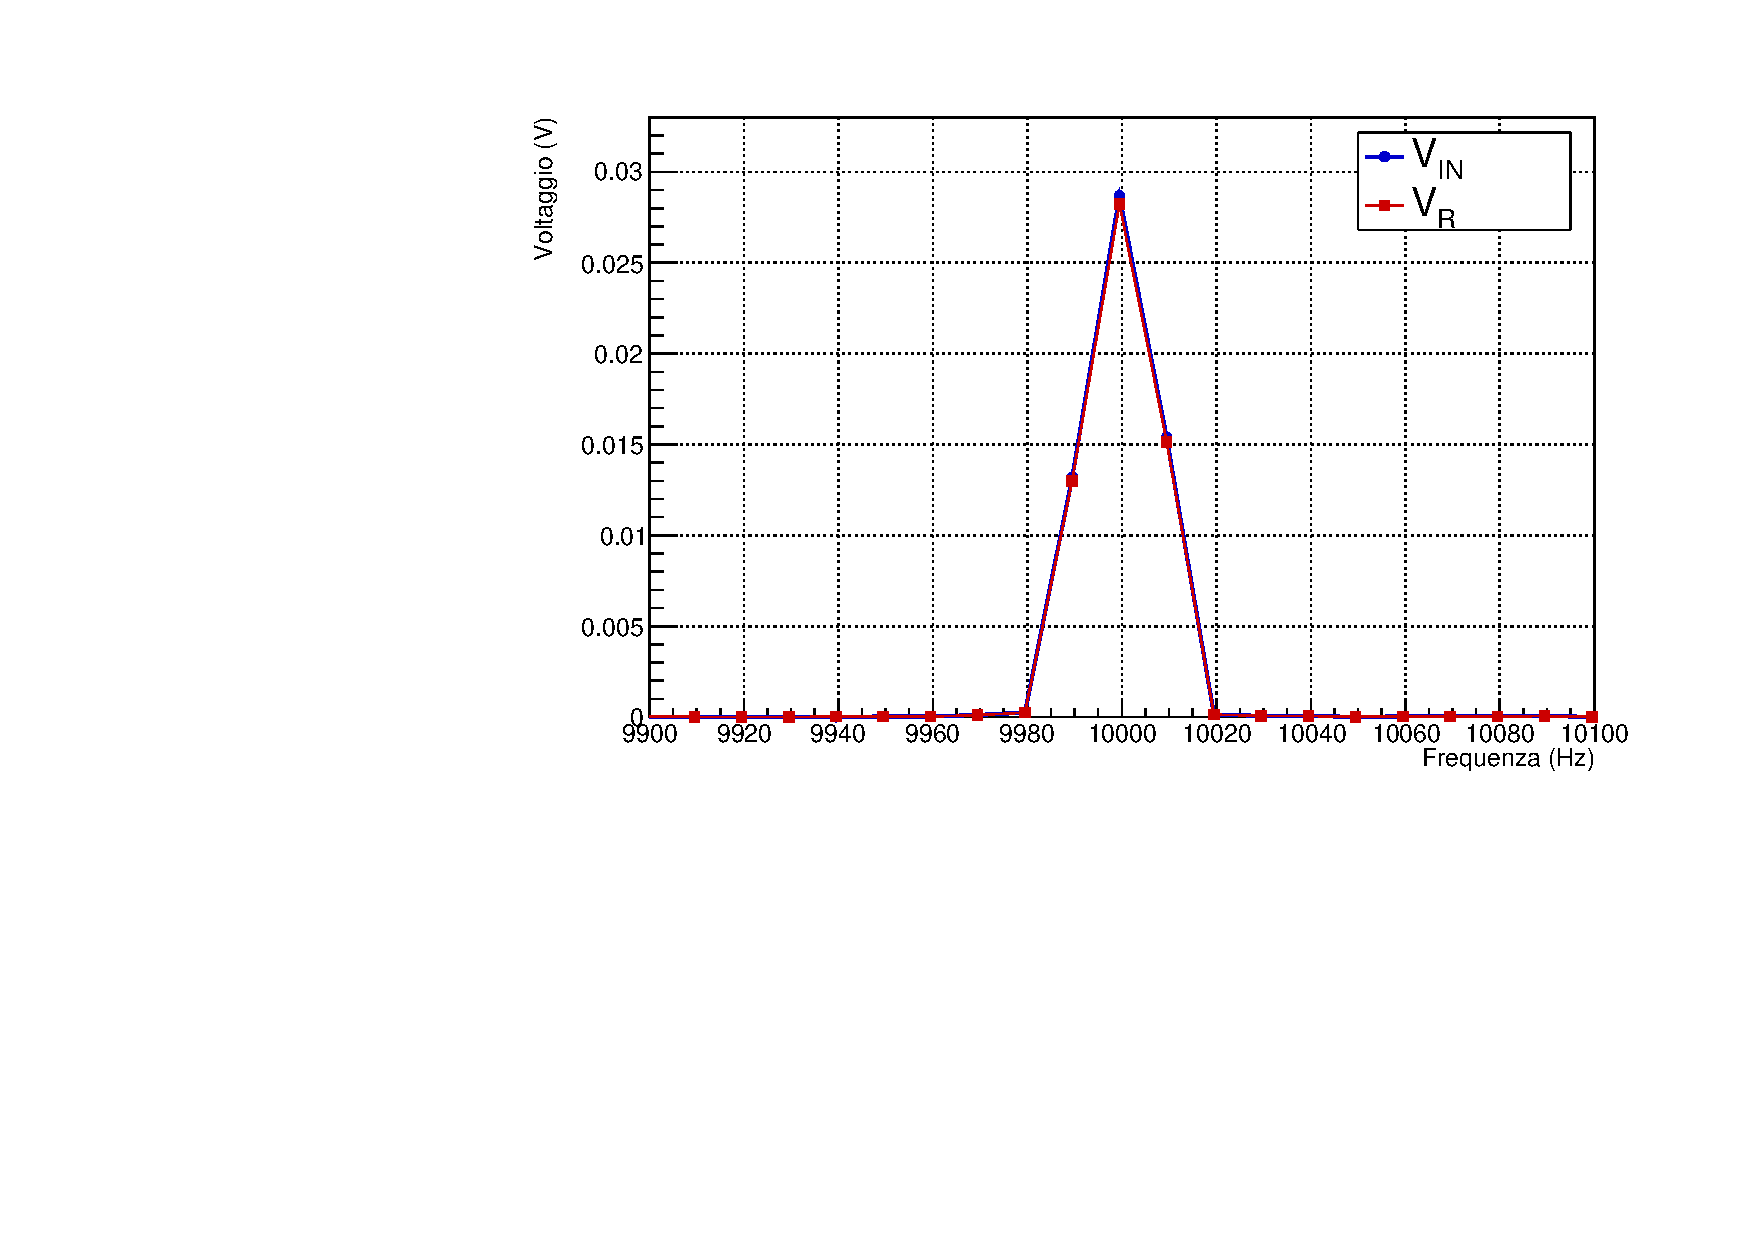
\includegraphics[width=\linewidth]{Images/Mic(10).pdf}
            \label{fig:3}
        \end{minipage}
    }
    \caption{.}
\end{figure}

Foto microfono a 7600, 2000, 10000 per confrontare

\section{Conclusioni}

Non faremo fisica sperimentale.

\section{Bibliografia}
Taylor, Prop Errori
Treccani
Libro di onde a caso

\section{Appendice}

\subsection{Incertezze Resistenze}
\label{app:Incertezze}
L'eq. 7.1 riporta il calcolo dell'incertezza associata ai valori di resistenza mediante multimetro della scheda Elvis II. Nella tabella 2 sono riportati i valori di range, errore sulla lettura e di fondo scala, per le corrispettive resistenze.

\begin{equation}
    Incertezza = \pm \left(\frac{Lettura*ppm_{Lettura}}{10^6}+\frac{Range*ppm_{Range}}{10^6}\right)
\end{equation}

\begin{table}[H]
\centering
\begin{tabular}{||c | c || c ||} 
 \hline
 Range & ppm della Lettura + ppm del Range  & Resistenze \\ [0.5ex] 
 \hline\hline
 100 $\Omega$ & 450 + 310 & 2.5 $\Omega$, 100 $\Omega$ \\
 \hline
 1 k$\Omega$ & 450 + 100 & 330 $\Omega$, 560 $\Omega$\\ 
 \hline
\end{tabular}
\caption{\textit{Estratto del manuale della scheda Elvis II. Sono riportati i valori di range, errore su lettura (ppm della Lettura) e di fondo scala (ppm del Range), e le corrispettive resistenze afferenti al range.}}
\end{table}

 A titolo esemplificativo, l'errore associato alla resistenza di 100 $\Omega$ è stato calcolato come:

\begin{equation}
    Incertezza_{100 \Omega} = \pm \left(\frac{450*100.31}{10^6}+\frac{310*100}{10^6}\right)
\end{equation}

\subsection{Equazione Fit}
\label{app:Dimostrazione}
\noindent Sono riportati i calcoli dell'eq. XXX


\begin{equation}
\begin{split}
    V(R) = R*I = R * \frac{V_0}{Z_{TOT}},
    \qquad \text{dove} \quad
    Z_{TOT} & = \left(\frac{1}{R_L + j\omega L} + j\omega L\right)^{-1} + R + R_V \\
    & = \left(\frac{R_L+j \omega L}{1 - \omega ^2 LC + j \omega C R_L}\right) + R + R_V \\
    & = \frac{R_L + j \omega L + (R + R_V) (1 - \omega ^2 L C + j \omega C R_L)}{1 - \omega ^2 L C + j \omega C R_L}    
\end{split}
\end{equation}

\begin{equation}
\begin{split}
    \text{Sostituendo $Z_{TOT}$,}  \quad
    V(R) & = R \cdot V_0 \frac{1-\omega ^2 L C + j \omega C R_L}{R_L + j \omega L + (R + R_V)(1 - \omega ^2 L C + j \omega C R_L)} \\
    & = V_0 \frac{R(1-\omega ^2 L C) + j R \omega C R_L}{[R_L + R + R_V -(R + R_V)(\omega ^2 L C)] + j [\omega L + (R + R_V) w C R_L]} \\
    & = |V_0| \frac{R \sqrt{(1-\omega ^2 L C)^2 + (\omega C R_L)^2}}{\sqrt{[(R_V + R) (1 - \omega ^2 L C ) + R_L]^2 + [\omega L + \omega C R_L ( R_V + R)]^2}} e^{i(\theta-\varphi)}
\end{split}
\end{equation}

\begin{equation}
    \text{Prendendone il modulo,} \quad
    |V(R)| =  |V_{0}| \frac{R \sqrt{(1-w^2LC)^2+(wCR_{L})^2}}{\sqrt{[(R_{V}+R)(1-w^2LC)+R_{L}]^2+\{w[L+CR_{L}(R_{V}+R)]\}^2}}
\end{equation}


\end{document}